\documentclass{beamer}

\usetheme{CambridgeUS}
\usecolortheme{dolphin}

\usepackage[utf8]{inputenc}
\usepackage[T1]{fontenc}

\usepackage{tikz}
\usetikzlibrary{3d}
\usepackage{xifthen}
\usepackage{tikzsymbols}
\usepackage{pgfplots}
\usepgfplotslibrary{fillbetween}
\usetikzlibrary{patterns}

\usepackage{listings}
\lstset{language=C,frame=single,basicstyle=\footnotesize\ttfamily}

\setbeamertemplate{sidebar right}{}
\setbeamertemplate{footline}{\hfill\usebeamertemplate***{navigation symbols}}


\addtobeamertemplate{navigation symbols}{}{%
\usebeamerfont{footline}%
\usebeamercolor[fg]{footline}%
\hspace{1em}%
\insertframenumber/\inserttotalframenumber
}


\begin{document}

\title{Optimising finite-difference methods for PDEs through parameterised time-tiling in Devito}
\subtitle{BEng JMC Individual Project}

\author{Nicholas Sim\\
~\\
{\normalsize Supervisors:}\\
Prof. Paul H. J. Kelly\\
Dr. Fabio Luporini\\
Sun Tianjiao}

\date{June 25, 2018}

\frame{\titlepage}



\section{Context}


\begin{frame}
\frametitle{Why solve differential equations?}

\begin{itemize}
	\item Some pictures
\end{itemize}
\end{frame}



\begin{frame}
\frametitle{Devito: solving differential equations quickly}
\begin{columns}
	\begin{column}{0.48\textwidth}
		\begin{itemize}
			\item DSL: forward/backward solution of PDEs
			\item Finite-difference methods work on structured grids
			\item Translation of PDEs to stencils to code
			\item Optimises stencils and code
			\item Related: OPS, stencil compilers
		\end{itemize}
	\end{column}
	\begin{column}{0.48\textwidth}

		\newcommand{\xangle}{11}
		\newcommand{\yangle}{133}
		\newcommand{\zangle}{270}

		\newcommand{\xlength}{1}
		\newcommand{\ylength}{1}
		\newcommand{\zlength}{1}

		\pgfmathsetmacro{\xx}{\xlength*cos(\xangle)}
		\pgfmathsetmacro{\xy}{\xlength*sin(\xangle)}
		\pgfmathsetmacro{\yx}{\ylength*cos(\yangle)}
		\pgfmathsetmacro{\yy}{\ylength*sin(\yangle)}
		\pgfmathsetmacro{\zx}{\zlength*cos(\zangle)}
		\pgfmathsetmacro{\zy}{\zlength*sin(\zangle)}

		\begin{center}
		\begin{tikzpicture}
		[   x={(\xx cm,\xy cm)},
		y={(\yx cm,\yy cm)},
		z={(\zx cm,\zy cm)},
		]

		\foreach \x in {3,2,1,0}
		{   \foreach \y in {3,2,1,0}
		{   \foreach \z in {4,3,2,1,0}
		{   \pgfmathsetmacro{\c}{100-(\x*\y*\z)/(3*3*4)*95}
		\ifthenelse{\x>0}
		{\draw[black!\c] (\x,\y,\z) -- (\x-1,\y,\z);}{}
		\ifthenelse{\y>0}
		{\draw[black!\c] (\x,\y,\z) -- (\x,\y-1,\z);}{}
		\ifthenelse{\z>0}
		{\draw[black!\c] (\x,\y,\z) -- (\x,\y,\z-1);}{}
		\fill[red!\c] (\x,\y,\z) circle (0.05cm);
		}
		}
		}

		\end{tikzpicture}
		\end{center}
	\end{column}
\end{columns}

\end{frame}



%\begin{frame}
%\frametitle{Target loops to optimise computation}
%
%\begin{itemize}
%	\item Loops: stepping through time iterations, problem domains
%	\item Large problem sets: weeks spent in loops
%	\item Optimise loops for speedup
%	\item We apply time-tiling, a \emph{loop nest optimisation}
%\end{itemize}
%\end{frame}



\begin{frame}
\frametitle{Time-tiling is a loop (nest) optimisation}

\begin{itemize}
	\item Loop nests: stepping through time, over 3 spatial dimensions
	\item \emph{Parameterisation} for auto-tuned optimisation
	\item Previous work: up to 27.5\% reduction\footnote{D.~McCormick. Applying the Polyhedral Model to Tile Loops in Devito. Master's thesis, Imperial College of Science, Technology and Medicine, 2017.}
	\item We get 36.8\% speedup for the \textbf{same} stencil
	\item Can achieve \(\ge 75\%\) of benchmarked memory bandwidth
\end{itemize}
\end{frame}



\begin{frame}
\frametitle{Contributions}

\begin{itemize}
	\item Implemented time-tiling in Devito
	\item Rigorous testing and numerical verification
	\item Evaluation of remaining implementation work
	\item Estimator for \emph{arithmetic intensity}, which helps identify bottlenecks
	\item Prediction of speedup from estimator
	\item Decrease runtime by 20--45\%!
	\newline
	\item Target delivery: next few months
	\item (How to present this simply?)
\end{itemize}
\end{frame}



\begin{frame}
\frametitle{This presentation}
\tableofcontents
\end{frame}



\section{Time-tiling in 5 minutes}

\begin{frame}
\frametitle{Stencils}

\begin{center}
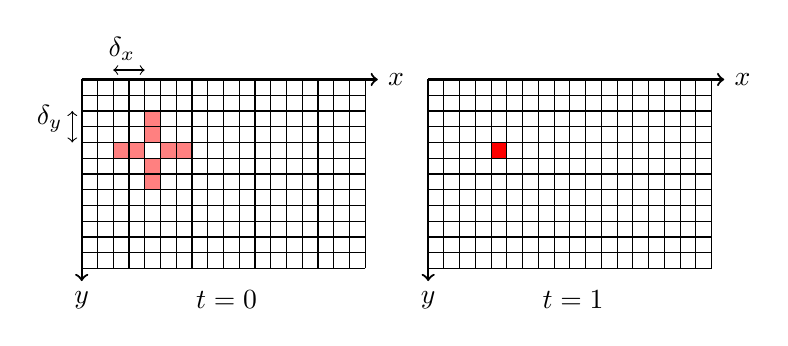
\begin{tikzpicture}[scale=.8]
\fill[red!50!white] (0.5,2) rectangle (1,1.75);
\fill[red!50!white] (1.25,2) rectangle (1.75,1.75);
\fill[red!50!white] (1,2.5) rectangle (1.25,2);
\fill[red!50!white] (1,1.25) rectangle (1.25,1.75);
\draw[xstep=.25cm,ystep=.25cm] (0,0) grid (4.5,3);
\draw[thick,->] (0,3) -- (4.7,3) node[right]{$x$};
\draw[thick,->] (0,3) -- (0,-.2) node[below]{$y$};
\draw (2.3,-.5) node {$t=0$};

\fill[red] (6.5,2) rectangle (6.75,1.75);
\draw[xstep=.25cm,ystep=.25cm] (5.5,0) grid (10,3);
\draw[thick,->] (5.5,3) -- (10.2,3) node[right]{$x$};
\draw[thick,->] (5.5,3) -- (5.5,-.2) node[below]{$y$};
\draw (7.8,-.5) node {$t=1$};

\draw[<->] (0.5,3.15) -- (1,3.15) node[above left]{$\delta_x$};
\draw[<->] (-.15,2.5) -- (-.15,2) node[above left]{$\delta_y$};
\end{tikzpicture}
\end{center}

\begin{itemize}
	\item Determine the value of a point
	\item Need values of neighbours in \emph{previous} time iteration
	\item \emph{Space-order} gives radius (\(\delta\))
\end{itemize}
\end{frame}

%\begin{frame}
%\frametitle{Non-problem: iteration space \(<\) cache size}
%
%\begin{center}
%	\begin{tikzpicture}[scale=.8]
%	\draw[blue,thick] (-1.5,4) rectangle (11.5,-2);
%	\draw (-.8,-1.7) node {Cache};
%
%	\fill[red!50!white] (0.5,2) rectangle (1,1.75);
%	\fill[red!50!white] (1.25,2) rectangle (1.75,1.75);
%	\fill[red!50!white] (1,2.5) rectangle (1.25,2);
%	\fill[red!50!white] (1,1.25) rectangle (1.25,1.75);
%	\draw[xstep=.25cm,ystep=.25cm] (0,0) grid (4.5,3);
%	\draw[thick,->] (0,3) -- (4.7,3) node[right]{$x$};
%	\draw[thick,->] (0,3) -- (0,-.2) node[below]{$y$};
%	\draw (2.3,-.5) node {$t=0$};
%
%	\fill[red] (6.5,2) rectangle (6.75,1.75);
%	\draw[xstep=.25cm,ystep=.25cm] (5.5,0) grid (10,3);
%	\draw[thick,->] (5.5,3) -- (10.2,3) node[right]{$x$};
%	\draw[thick,->] (5.5,3) -- (5.5,-.2) node[below]{$y$};
%	\draw (7.8,-.5) node {$t=1$};
%	\end{tikzpicture}
%\end{center}
%
%\begin{itemize}
%	\item If iteration space \(<\) cache, no need to reload data
%	\item Everything loaded once \Smiley
%\end{itemize}
%\end{frame}



%\begin{frame}
%\frametitle{Problem: iteration space \(>\) cache size}
%
%\begin{center}
%	\begin{tikzpicture}[scale=.8]
%	\fill[red!50!white] (0.5,2) rectangle (1,1.75);
%	\fill[red!50!white] (1.25,2) rectangle (1.75,1.75);
%	\fill[red!50!white] (1,2.5) rectangle (1.25,2);
%	\fill[red!50!white] (1,1.25) rectangle (1.25,1.75);
%	\draw[xstep=.25cm,ystep=.25cm] (0,0) grid (4.5,3);
%	\draw[thick,->] (0,3) -- (4.7,3) node[right]{$x$};
%	\draw[thick,->] (0,3) -- (0,-.2) node[below]{$y$};
%	\draw (2.3,-.5) node {$t=0$};
%
%	\fill[red] (6.5,2) rectangle (6.75,1.75);
%	\draw[xstep=.25cm,ystep=.25cm] (5.5,0) grid (10,3);
%	\draw[thick,->] (5.5,3) -- (10.2,3) node[right]{$x$};
%	\draw[thick,->] (5.5,3) -- (5.5,-.2) node[below]{$y$};
%	\draw (7.8,-.5) node {$t=1$};
%
%	\draw[blue,thick] (-.125,2.375) rectangle (2.125,1.375);
%	\draw (-1,1.7) node {Cache};
%	\end{tikzpicture}
%\end{center}
%
%\begin{itemize}
%	\item Load neighbours (t=0) into cache, some reuse in t=1 row
%	\item Evicted by the time we reach end of row
%	\item Poor cache usage: need to load rows again
%	\item Everything loaded 3 times \Sadey
%\end{itemize}
%\end{frame}



%\begin{frame}
%\frametitle{Solution: pretend iteration space \(<\) cache size}
%
%\begin{center}
%	\begin{tikzpicture}[scale=.8]
%	\fill[red!30!white] (0,1.25) rectangle (4.5,1.75);
%	\fill[red!30!white] (0.25,0) rectangle (.75,3);
%	\fill[red!30!white] (1.75,0) rectangle (2.25,3);
%	\fill[red!30!white] (3.25,0) rectangle (3.75,3);
%	\draw[xstep=.125cm,ystep=.125cm,thin] (0,0) grid (4.5,3);
%	\draw[thick,->] (0,3) -- (4.7,3) node[right]{$x$};
%	\draw[thick,->] (0,3) -- (0,-.2) node[below]{$y$};
%	\draw (2.3,-.5) node {$t=0$};
%
%	\draw[xstep=.125cm,ystep=.125cm,thin] (5.5,0) grid (10,3);
%	\draw[thick,->] (5.5,3) -- (10.2,3) node[right]{$x$};
%	\draw[thick,->] (5.5,3) -- (5.5,-.2) node[below]{$y$};
%	\draw (7.8,-.5) node {$t=1$};
%	\draw[red,thick,xstep=1.5cm,ystep=1.5cm] (5.3,-.2) grid (10.2,3.2);
%
%	\draw[blue,thick] (-.05,3.05) rectangle (2.15,1.35);
%	\end{tikzpicture}
%\end{center}
%
%\begin{itemize}
%	\item Insight: x,y can be calculated in any order (parallel!)
%	\item Partition into \emph{tiles}
%	\item Only tile boundaries loaded twice
%	\item `Exploiting data locality'
%\end{itemize}
%\end{frame}



\begin{frame}
\frametitle{When tiling (doesn't) work}

\begin{itemize}
	\item If memory bounded, less data transfer \(\rightarrow\) faster
	\item If compute bounded, optimising cache doesn't help much...
	\item Can make compute bounded stencils more memory bounded\footnote{F. Luporini et al. An Algorithm for the Optimisation of Finite Element Integration Loops. \emph{ACM Trans. on Math. Software}, 44(1):1--26, Mar 2017.}
	\newline
	\item We needed to be able to permute x and y
	\item But can only take 1 time step at a time
	\item Instead, interchange time and space loops and proceed sequentially
	\item (Distribute this)
	\item (redo diagrams for 1d)
\end{itemize}
\end{frame}



\begin{frame}
\frametitle{Can't interchange these loops}

\begin{center}
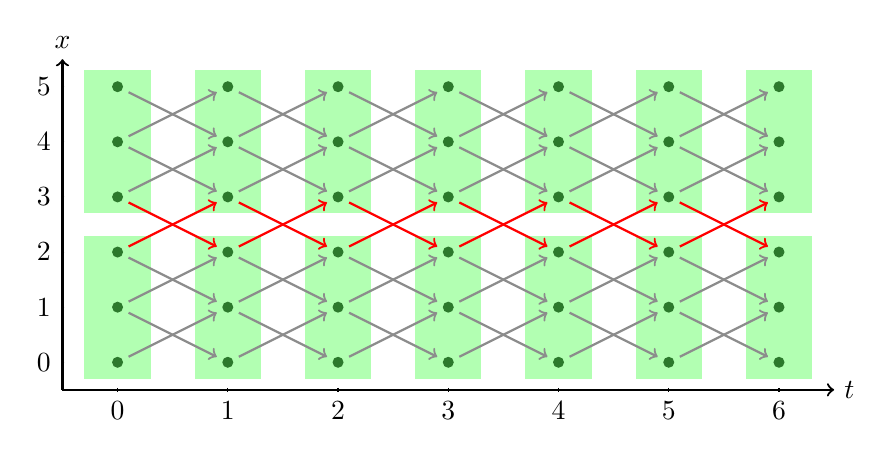
\begin{tikzpicture}[scale=0.7]
\draw[thick,->] (-1,-.5) -- (13,-.5) node[right]{$t$};
\draw[thick,->] (-1,-.5) -- (-1,5.5) node[above]{$x$};

\foreach \t in {0,1,2,3,4,5,6}
\foreach \x in {0,1,2,3,4,5}
\fill[darkgray] (\t*2,\x) circle (0.1);

\foreach \t in {0,1,2,3,4,5,6}
\foreach \x in {0,3}
\fill[green,opacity=0.3] (\t*2-.6,\x-.3) rectangle (\t*2+.6,\x+2.3);

\foreach \t in {0,1,2,3,4,5}
\foreach \x in {1,2,4,5}
\draw[thick,->,darkgray!60] (\t*2+.2,\x-.1) -- (\t*2+1.8,\x-.9);
\foreach \t in {0,1,2,3,4,5}
\foreach \x in {3}
\draw[thick,->,red] (\t*2+.2,\x-.1) -- (\t*2+1.8,\x-.9);

\foreach \t in {0,1,2,3,4,5}
\foreach \x in {0,1,3,4}
\draw[thick,->,darkgray!60] (\t*2+.2,\x+.1) -- (\t*2+1.8,\x+.9);
\foreach \t in {0,1,2,3,4,5}
\foreach \x in {2}
\draw[thick,->,red] (\t*2+.2,\x+.1) -- (\t*2+1.8,\x+.9);

\foreach \t in {0,1,2,3,4,5,6}
\draw (\t*2,1pt-.5cm) -- (\t*2,-1pt-.5cm) node[anchor=north] {$\t$};
\foreach \x in {0,1,2,3,4,5}
\draw (1pt-1cm,\x) -- (-1pt-1cm,\x) node[anchor=east] {$\x$};
\end{tikzpicture}
\end{center}

\begin{itemize}
	\item Dependencies between rows flow two ways
\end{itemize}
\end{frame}



\begin{frame}
\frametitle{Idea: skewed tiling for interchange}

\begin{center}
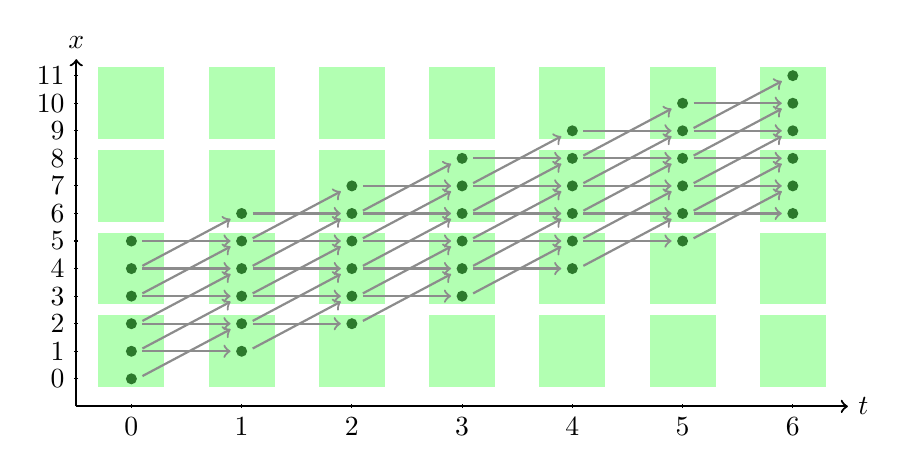
\begin{tikzpicture}[scale=0.7]
\draw[thick,->] (-1,-.5) -- (13,-.5) node[right]{$t$};
\draw[thick,->] (-1,-.5) -- (-1,5.8) node[above]{$x$};

\foreach \t in {0,1,2,3,4,5,6}
\foreach \x in {0,1,2,3,4,5}
\fill[darkgray] (\t*2,\x/2+\t/2) circle (0.1);

\foreach \t in {0,1,2,3,4,5,6}
\foreach \x in {0,3,6,9}
\fill[green,opacity=0.3] (\t*2-.6,\x/2-.15) rectangle (\t*2+.6,\x/2+1.15);

\foreach \t in {0,1,2,3,4,5}
\foreach \x in {1,2,3,4,5}
\draw[thick,->,darkgray!60] (\t*2+.2,\x/2+\t/2) -- (\t*2+1.8,\x/2+\t/2);

\foreach \t in {0,1,2,3,4,5}
\foreach \x in {0,1,2,3,4}
\draw[thick,->,darkgray!60] (\t*2+.2,\x/2+\t/2+.05) -- (\t*2+1.8,\x/2+\t/2+.9);

\foreach \t in {0,1,2,3,4,5,6}
\draw (\t*2,1pt-.5cm) -- (\t*2,-1pt-.5cm) node[anchor=north] {$\t$};
\foreach \x in {0,1,2,3,4,5,6,7,8,9,10,11}
\draw (1pt-1cm,\x/2) -- (-1pt-1cm,\x/2) node[anchor=east] {$\x$};
\end{tikzpicture}
\end{center}

\begin{itemize}
	\item Less transfer: if a tile fits in cache, can calculate subsequent tiles in that row from cache \Smiley
\end{itemize}
\end{frame}



%\begin{frame}[fragile]
%\frametitle{Time-tiling: some important details}
%
%\begin{itemize}
%	\item Minimum skew: the distance of the spatial dependence
%	\item Out of bounds accesses
%	\item Only works for perfect loop nests
%\end{itemize}
%\begin{lstlisting}
%// Imperfect loop nest
%
%for (int t = t_s; t < t_e; t++) {
%  for (int x = x_s; x < x_e; x++)
%    for (int y = y_s; y < y_e; y++)
%      A[t][x][y] = A[t-1][x-1][y+1] + A[t-1][x+1][y-1];
%  for (int j = j_s; j < j_e; j++)
%    A[t][j][j+1] *= 1.5;
%}
%\end{lstlisting}
%\end{frame}



%\begin{frame}
%\frametitle{Testing framework}
%
%\begin{itemize}
%	\item CSG Intel Xeon E5-2470; 8 cores, 16 threads, 20MB L3 cache
%	\item 64GB DRAM
%	\item OpenMP: parallelism, use all threads, prevent migration
%	\item Intel C Compiler, all optimisations enabled
%	\item Devito auto-tuner to ensure best runtime
%	\item Always verify functional correctness
%	\item Minimum runtime reported
%	\item (small print on diagrams)
%\end{itemize}
%\end{frame}



\section{Results}

\begin{frame}
\frametitle{Evaluation}

\begin{itemize}
	\item 9 stencils from acoustic wave equation, Laplace operators
	\item All results numerically exact
	\item Auto-tuning: search for fastest tile sizes (parameterised)
	\newline
	\item Qn: how effective is time-tiling and when?
\end{itemize}
\end{frame}



\begin{frame}
\frametitle{Speedup decreases with increasing arith. intensity\footnote{\tiny Min. runtime reported: data numerically verified, tile sizes auto-tuned. Tested on Intel Xeon E5-2470; 8 cores, 16 threads, 64GB DRAM. OpenMP for parallelism, no migration on 16 threads; compilation \texttt{icc -qopenmp -O3 ...}}}
\vspace{-3em}
\begin{columns}
\begin{column}{.49\textwidth}
\begin{center}
\begin{tikzpicture}[scale=.51]
\begin{axis}[
width=2\textwidth,
xlabel={Space order (AWE)},
xtick distance=1,
symbolic x coords={4,6,8,12,16},
nodes near coords,
axis y line*=left,
ylabel near ticks, yticklabel pos=right,
ylabel={Speedup vs non-tiled (\(1\times\))},
ymin=0, ymax=4,
ybar,
every node near coord/.append style={font=\fontsize{6.5}{6.5}},
]
\addplot table [x=sp,y=run,col sep=comma] {../data/awe-nt512.csv};
\addplot table [x=sp,y=run,col sep=comma] {../data/awe-sp512.csv};
\addplot table [x=sp,y=run,col sep=comma] {../data/awe-tm512.csv};
\end{axis}

\begin{axis}[
width=2\textwidth,
legend style={at={(.02,.98)},anchor=north west},
axis y line*=right,
ylabel near ticks, yticklabel pos=right,
axis x line=none,
%ylabel={Arith. intensity},
ybar,
symbolic x coords={4,6,8,12,16},
ymin=0, ymax=16,
]
\addplot[smooth,mark=*,blue]
coordinates{
	(4,2.1)
	(6,2.5)
	(8,2.89)
	(12,3.36)
	(16,4.42)
};
\legend{Arith. intensity (spatial tiling)}
\end{axis}
\end{tikzpicture}
\end{center}
\end{column}

\begin{column}{.49\textwidth}
\begin{center}
\begin{tikzpicture}[scale=.51]
\begin{axis}[
width=2\textwidth,
legend style={at={(.02,.98)},anchor=north west},
xlabel={Space order (Laplace)},
xtick distance=1,
symbolic x coords={2,4,8,16},
nodes near coords,
axis y line*=left,
ylabel near ticks, yticklabel pos=right,
%ylabel={Speedup vs non-tiled (\(1\times\))},
ymin=0, ymax=4,
ybar,
every node near coord/.append style={font=\fontsize{6.5}{6.5}},
]
\addplot table [x=sp,y=run,col sep=comma] {../data/laplace-nt600.csv};
\addplot table [x=sp,y=run,col sep=comma] {../data/laplace-sp600.csv};
\addplot table [x=sp,y=run,col sep=comma] {../data/laplace-tm600.csv};
\legend{Non-tiled,Space-tiling,Time-tiling}
\end{axis}

\begin{axis}[
width=2\textwidth,
axis y line*=right,
ylabel near ticks, yticklabel pos=right,
axis x line=none,
symbolic x coords={2,4,8,16},
ymin=0, ymax=16,
ylabel={Arith. intensity},
ybar,
]
\addplot[smooth,mark=*,blue]
coordinates{
	(2,4.69)
	(4,6.31)
	(8,9.29)
	(16,14.0)
};
\end{axis}
\end{tikzpicture}
\end{center}
\end{column}
\end{columns}

\begin{itemize}
	\item Speedup (vs spatial tiling) greatest with high memory pressure
	\item Near computational bound \(\rightarrow\) marginal improvement
\end{itemize}
\end{frame}



\begin{frame}
\frametitle{Arithmetic intensity: time-tiling decreases memory transfer}

\begin{itemize}
	\item Floating point operations per byte transferred from memory
	\item More operations \(\rightarrow\) more computational resources needed
	\item Fewer operations \(\rightarrow\) more memory bandwidth needed
	\newline
	\item Time-tiling increases arithmetic intensity
	\item Constructed an estimator to measure this
\end{itemize}
\end{frame}



\begin{frame}
\frametitle{Roofline model\footnote{\tiny S. Williams et al. Roofline: An insightful visual performance model for multicore architectures. \emph{Commun. ACM}, April 2009.\\LINPACK: J. Dongarra. Performance of various computers using standard linear equations software. Tech. report, Knoxville TN, 1989.\\STREAM: J. McCalpin. Memory bandwidth and machine balance in current high performance computers. \emph{IEEE Computer Society TCCA Newletter}, Dec 1995.} to understand performance}

\begin{columns}
\begin{column}{0.48\textwidth}
\begin{center}
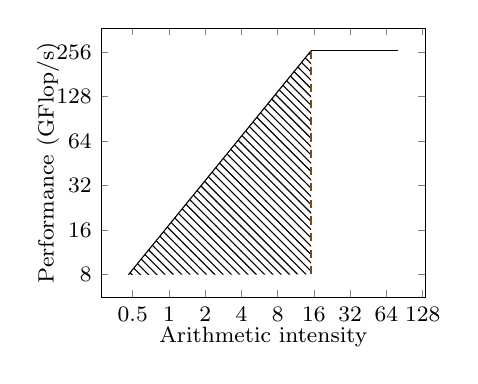
\begin{tikzpicture}[scale=.6]
\begin{axis}[
legend style={at={(0.95,0.05)},anchor=south east},
xlabel={Arithmetic intensity},
ylabel={Performance (GFlop/s)},
domain=0.4:96,
xmode=log,
log basis x={2},
ymode=log,
log basis y={2},
log ticks with fixed point,
tick label style={font=\footnotesize},
label style={font=\footnotesize}
]
% roofline
\addplot [domain=0.46:15.15,name path=A] {17.3*x};
\addplot [domain=15.15:80] {262.01};
% boundary
%\path[name path=X] (axis cs:15.5,8) -- (axis cs:15.5,262.01);
\addplot +[mark=none,dashed,thick,name path=X] coordinates {(15.15, 8) (15.15, 262.01)};
\addplot[gray, pattern=north west lines] fill between [of=A and X];
\end{axis}
\end{tikzpicture}
\end{center}
\end{column}
\begin{column}{0.48\textwidth}
	\begin{itemize}
		\item Memory bounded (shaded), then CPU bounded
		\item LINPACK: 262 GFlops
		\item STREAM: 17.3 GB/s
		\item Can't exceed roofline: overestimate arithmetic intensity
	\end{itemize}
\end{column}
\end{columns}
\end{frame}



\begin{frame}
\frametitle{Roofline: still memory bounded;\footnote{\tiny Min. runtime reported: data numerically verified, tile sizes auto-tuned. Tested on Intel Xeon E5-2470; 8 cores, 16 threads, 64GB DRAM. OpenMP for parallelism, no migration on 16 threads; compilation \texttt{icc -qopenmp -O3 ...}} finding ideal time tile sizes}
\vspace{-2em}
\begin{columns}
\begin{column}{.49\textwidth}
\begin{center}
\begin{tikzpicture}[scale=.51]
\begin{axis}[
width=2\textwidth,
legend style={at={(.95,.05)},anchor=south east},
xlabel={Arithmetic intensity (AWE)},
ylabel={Performance (GFlop/s)},
xmode=log,
log basis x={2},
ymode=log,
ymin=24, ymax=68,
log basis y={2},
log ticks with fixed point,
cycle list name=exotic,
]
\addplot table [x=oi,y=gflops,col sep=comma] {../data/awe-roof-so16.csv};
\addplot table [x=oi,y=gflops,col sep=comma] {../data/awe-roof-so12.csv};
\addplot[mark=triangle] table [x=oi,y=gflops,col sep=comma] {../data/awe-roof-so8.csv};
\addplot table [x=oi,y=gflops,col sep=comma] {../data/awe-roof-so6.csv};
\addplot[blue,mark=diamond] table [x=oi,y=gflops,col sep=comma] {../data/awe-roof-so4.csv};

\addplot [domain=1.5:5] {17.3*x};
%\addplot [domain=15.15:150] {262.01};
\addplot [domain=2:5,dashed] {13*x};
\legend{Time-tiling so16,Time-tiling so12, Time-tiling so8,Time-tiling so6, Time-tiling so4}
\end{axis}
\end{tikzpicture}
\end{center}
\end{column}

\begin{column}{.49\textwidth}
\begin{center}
\begin{tikzpicture}[scale=.51]
\begin{axis}[
width=2\textwidth,
legend style={at={(.95,.92)},anchor=north east},
xlabel={Arithmetic intensity (Laplace)},
ylabel={Performance (GFlop/s)},
xmode=log,
log basis x={2},
ymode=log,
ymin=30, ymax=280,
log basis y={2},
log ticks with fixed point,
cycle list name=exotic,
]
\addplot table [x=oi,y=gflops,col sep=comma] {../data/laplace-roof-so16.csv};
\addplot table [x=oi,y=gflops,col sep=comma] {../data/laplace-roof-so8.csv};
\addplot[mark=triangle] table [x=oi,y=gflops,col sep=comma] {../data/laplace-roof-so4.csv};
\addplot table [x=oi,y=gflops,col sep=comma] {../data/laplace-roof-so2.csv};
\legend{Time-tiling so16,Time-tiling so8,Time-tiling so4,Time-tiling so2}
% roofline
\addplot [domain=2:15.15,name path=A] {17.3*x};
\addplot [domain=15.15:50] {262.01};
\end{axis}
\end{tikzpicture}
\end{center}
\end{column}
\end{columns}

\begin{itemize}
%	\item Bottom-to-top: increasing time tile sizes
	\item Estimator much stronger with large time tiles (smaller overestimate)
	\item Larger time tiles \(\rightarrow\) usually faster
	\item Convergence: reached maximum cache reuse from time-tiling
\end{itemize}
\end{frame}



\begin{frame}
\frametitle{Effect of time tile size}

\begin{itemize}
	\item Low space order: big time tiles
	\item High space order: not much benefit after tile sizes 4, 8
	\item Non-trivial tile boundary overlap and finite cache \(\rightarrow\) arithmetic intensity overestimated
\end{itemize}
\end{frame}



\begin{frame}
\frametitle{Effect of skewing factor}

\begin{itemize}
	\item No change to arith. intensity
	\item (I didn't include the tables: should I?)
	\item Smallest valid skewing factor is fastest: even 3, 6
	\item Possibly because we need to load the neighbours anyway, so misalignment not an issue
\end{itemize}
\end{frame}



\begin{frame}
\frametitle{Further evaluation work and limitations}

\begin{itemize}
	\item Implementation -- only perfect loops
	\item Test more architectures
	\item Analyse memory to check cache misses, new bottlenecks
	\item Applications of the arithmetic intensity estimator
	\item Changed the spatial tiling algorithm slightly
	\item Multistep approximations
\end{itemize}
\end{frame}



\section{Conclusion}

\begin{frame}
\frametitle{Conclusion}

\begin{itemize}
	\item Contributions
	\item (move discussion of further work here?)
	\item What else?
\end{itemize}
\end{frame}



%\begin{frame}
%\frametitle{}
%
%\begin{itemize}
%	\item 
%	\item 
%	\item 
%	\item 
%\end{itemize}
%\end{frame}


\end{document}